\subsection{OSI参照モデル}

インターネットで利用されるプロトコルは、The Internet Engineering Task Force (IETF)という標準化
団体により策定され、その標準はRequest for Comments (RFC)という名のオープンな仕様として発行されている。
例えば、我々が利用しているインターネットプロトコルである
インターネットプロトコル バージョン4は、1981年に791番目のRFCとして策定された~\cite{RFC0791}。

IETF以外の通信に関する標準化団体としては
International Telecommunication Union Telecommunication Standardization Sector (ITU-T)や、
International Organization for Standardization (ISO)が存在する。
実は、1977年から1982年かけて、ITU-TやISOがコンピュータネットワークの標準通信プロトコルとして、
Open Systems Interconnection (OSI)の策定を行っていた。
その当時は標準的な通信プロトコルは存在せず、ベンダーごとに様々なプロトコルが利用されていたため、
通信プロトコルの統一化が求められていたのである。
しかしながら、最終的にOSIは主流とはならず、IETFによって策定された
インターネットプロトコルが広く利用されるようになっていった。

\begin{figure}[tb]
    \centering
    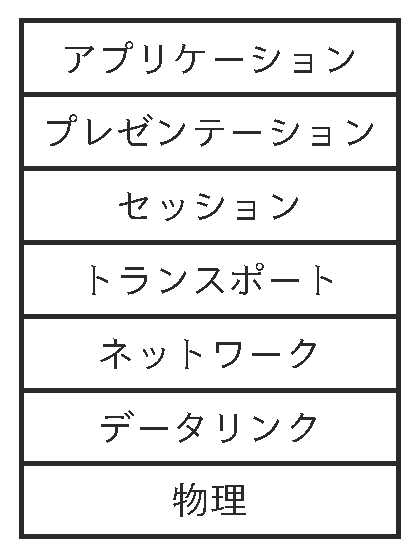
\includegraphics[width=5cm,pagebox=artbox]{figs/OSI.pdf}
    \caption{OSI参照モデル}
    \label{fig:osi}
\end{figure}

OSI自体は残らなかったが、OSI策定の際に考案されたOSI参照モデルと呼ばれる
ネットワークの抽象化手法は、今日でも広く受け入れられている。
図~\ref{fig:osi}は、OSI参照モデルによるネットワークの抽象化モデルを表している。
OSI参照モデルでは、ネットワークの機能を階層構造にもとづいて抽象化しており、
この抽象化をレイヤリングなどと呼ぶ。
OSI参照モデルでは、下から順に1層に物理層、2層にデータリンク層、
3層にネットワーク層、4層にトランスポート層、5層にセッション層、
6層にプレゼンテーション層、7層にアプリケーション層が位置する。
ちなみに、各層のことをレイヤ1、レイヤ2といったり、更に略してL1、L2などということもある。

\begin{figure}[tb]
    \centering
    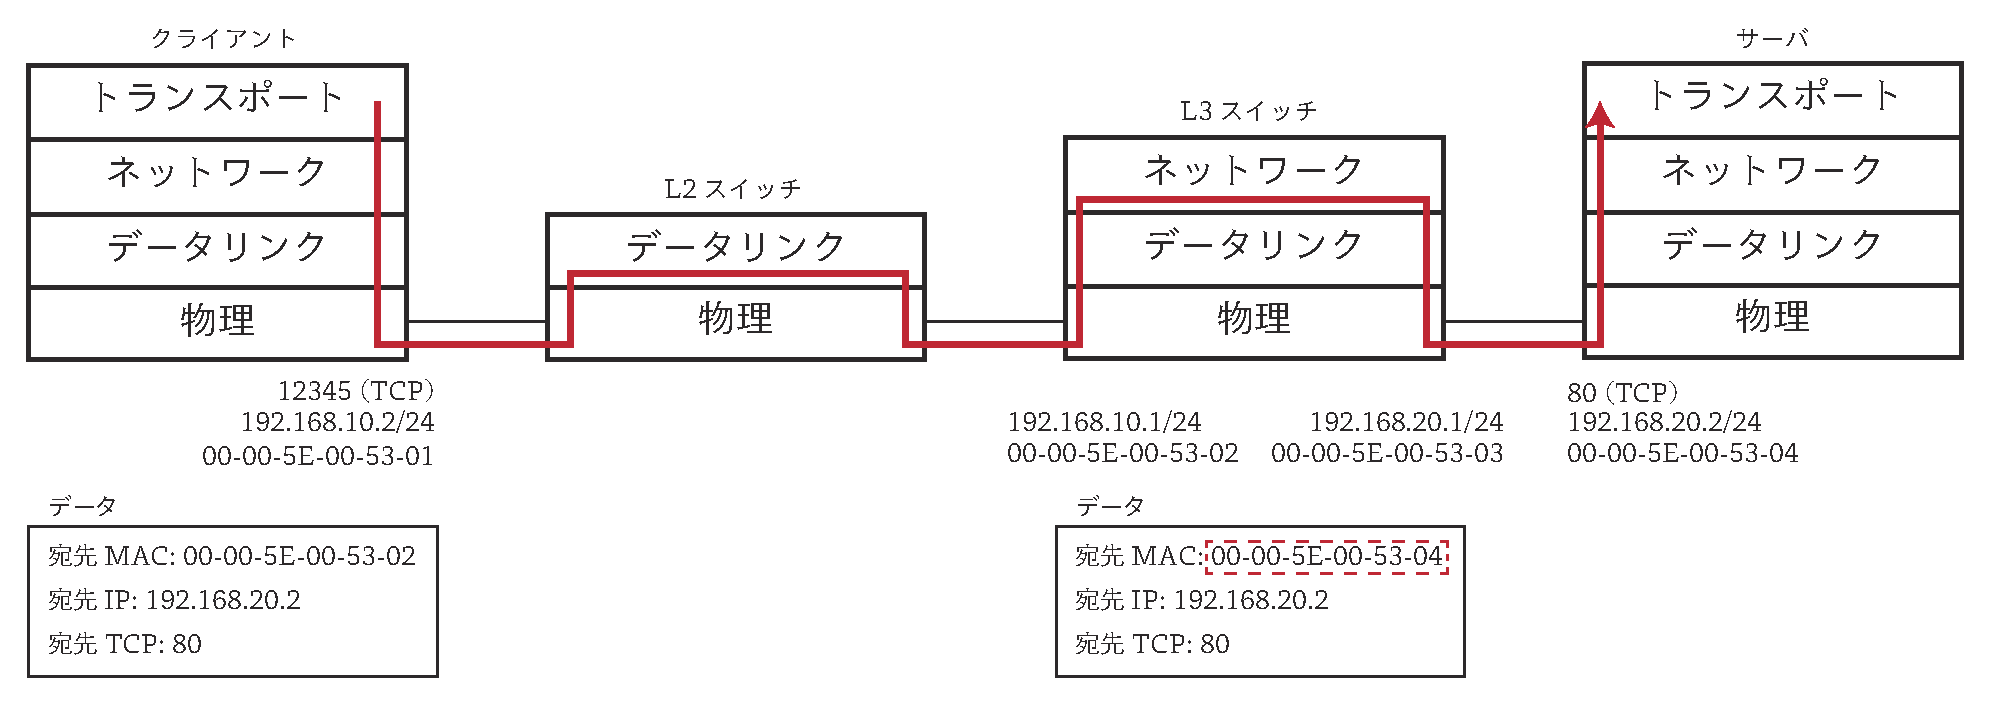
\includegraphics[width=14cm,pagebox=artbox]{figs/osi_link.pdf}
    \caption{各層でのデータ転送}
    \label{fig:osi_link}
\end{figure}

図~\ref{fig:osi_link}は各層でデータ転送が行われている様子を示している。
\footnote{
この図の意味することは現時点では理解できないかもしれないが、
この図の意味することろを説明するのが本節の目標であるため、
現段階で理解できなくても問題ない。
}
データリンク、ネットワーク、トランスポート層のプロトコルにはそれぞれアドレスがあり、
各層は、そのアドレスに基づいて転送を行う。
データリンク層プロトコルの一つであるIEEE 802では、アドレスは42ビットで表され、文字で表現すると00-00-5E-00-53-02といった
表記になる。
図~\ref{fig:osi_link}中で宛先MACと示される値は、
IEEE 802の宛先MACアドレスを示している。
なお、MACは Media Access Controlの略である。
データリンク層は、ローカルなネットワークでの通信を行うために用いられる。
そのため、MACアドレスはそのローカルな環境では一意に識別できる必要がある。
データリンク層の詳細については~\ref{sec:datalink}節で解説する。

ネットワーク層プロトコルの一つであるIPのアドレスは、192.168.10.2/24という32ビットの数値で表され、
/24はネットワークのサブネット長を示している。
図~\ref{fig:osi_link}では、192.168.10.0/24と192.168.20.0/24
というサブネットが示されている。
IPは、全世界で通信を行うために用いられるプロトコルであり、
基本的にはIPアドレスは世界で一意に識別できるように割り当てるのが設計理念となっている
(現実的にはそうはなっていないが)。
なお、前述のアドレスはIPv4アドレスであるが、IPv6の場合は128ビットのアドレス空間を持つ。
ネットワーク層の詳細については~\ref{sec:network}節で解説する。

トランスポート層プロトコルのTCPとUDPのアドレスは16ビットで示され、一般的にポート番号と呼ばれ、
TCPやUDPはポート番号をもとにアプリケーションプロセスの識別を行う。
よく利用されるポート番号は、インターネット上で利用される識別情報の管理割当を行っている
Internet Assigned Number Authority (IANA)が定義しており~\cite{wellknown}、
一般的にこのようなポート番号をWell Knownポート番号と呼ぶ。
例えば、TCPの80番ポートはHTTPで利用され、普段我々がWebを閲覧する際は、
WebブラウザがWebサーバのTCP80番ポートへ接続する。

図~\ref{fig:osi_link}では、クライントからサーバのTCP80番ポートへむけて
通信を行っている様子を示している。
一般的に、インターネット上の通信ではデータ中に含まれる各層のアドレスをもとに、
L2またはL3スイッチが転送を行う。
L2スイッチのことをスイッチングハブといったり、
L3スイッチのことをルータということもあるが、本書ではL2スイッチ、
L3スイッチと呼ぶことにする。
この図が示すように、L2スイッチ、L3スイッチによってデータが転送されても、
データ中のIPアドレスとポート番号は変わらないが、MACアドレスはL3スイッチでの転送時に更新される。
これは、MACアドレスはローカルなネットワーク内でのみ通用するアドレスであり、
L3スイッチはローカルなネットワーク同士をつなぎ合わせる役割を持っているためである。
以降の節では、データリンク、ネットワーク、トランスポートの動きについて詳しく説明する。

\begin{itembox}[l]{\bf 重要ポイント}
    \begin{itemize}
        \item インターネット関連のプロトコルは、IETFが発行するRFCによって標準化されている
        \item コンピュータネットワークはレイヤで考えることができる
        \item Ethernetのアドレスは48ビットのMACアドレス、IPv4のアドレスは32ビットのIPv4アドレス、IPv6のアドレスは128ビットのIPv6アドレス、TCPとUDPのアドレスは16ビットのポート番号
    \end{itemize}
\end{itembox}

\subsection{データリンク層} \label{sec:datalink}

\begin{lstlisting}[caption=Ethernetプロトコルヘッダ定義 (/usr/include/netinet/if\_ether.h),label=src:if_ether.h]
#define ETHER_ADDR_LEN  6       /* Ethernet address length              */

/*
 * Ethernet address - 6 octets
 */
struct ether_addr {
        u_int8_t ether_addr_octet[ETHER_ADDR_LEN];
};

/*
 * The length of the combined header.
 */
struct  ether_header {
        u_int8_t  ether_dhost[ETHER_ADDR_LEN];
        u_int8_t  ether_shost[ETHER_ADDR_LEN];
        u_int16_t ether_type;
};
\end{lstlisting}


\begin{lstlisting}[caption=Ethernet入力 (/usr/include/netinet/if\_ether.h),label=src:if_ether]
void ether_input(struct ether_header *eh)
{
    if (memcmp(eh->ether_dhost, my_ether_addr, ETHER_ADDR_LEN)) {
        bridge_input(eh);
        return;
    }

    switch (eh->ether_type) {
    case ETHERTYPE_IP:
        ipv4_input(&eh[1]);
        break;
    case ETHERTYPE_IP6:
        ipv6_input(&eh[1]);
        break;
    default:
        return;
    }

    return;
}
\end{lstlisting}


\subsection{ネットワーク層} \label{sec:network}

\begin{lstlisting}[caption=IPv4ヘッダ定義 (/usr/include/netinet/ip.h),label=src:ip.h]
/*
 * Structure of an internet header, naked of options.
 */
struct ip {
#if _BYTE_ORDER == _LITTLE_ENDIAN
        u_int     ip_hl:4,              /* header length */
                  ip_v:4;               /* version */
#endif
#if _BYTE_ORDER == _BIG_ENDIAN
        u_int     ip_v:4,               /* version */
                  ip_hl:4;              /* header length */
#endif
        u_int8_t  ip_tos;               /* type of service */
        u_int16_t ip_len;               /* total length */
        u_int16_t ip_id;                /* identification */
        u_int16_t ip_off;               /* fragment offset field */
#define IP_RF 0x8000                    /* reserved fragment flag */
#define IP_DF 0x4000                    /* dont fragment flag */
#define IP_MF 0x2000                    /* more fragments flag */
#define IP_OFFMASK 0x1fff               /* mask for fragmenting bits */
        u_int8_t  ip_ttl;               /* time to live */
        u_int8_t  ip_p;                 /* protocol */
        u_int16_t ip_sum;               /* checksum */
        struct    in_addr ip_src, ip_dst; /* source and dest address */
};
\end{lstlisting}

\begin{lstlisting}[caption=IPv6アドレス構造体 (/usr/include/netinet6/in6.h),label=src:in6.h]
/*
 * IPv6 address
 */
struct in6_addr {
        union {
                u_int8_t   __u6_addr8[16];
                u_int16_t  __u6_addr16[8];
                u_int32_t  __u6_addr32[4];
        } __u6_addr;                    /* 128-bit IP6 address */
};
\end{lstlisting}

\begin{lstlisting}[caption=IPv6ヘッダ定義 (/usr/include/netinet/ip6.h),label=src:ip6.h]
/*
 * Definition for internet protocol version 6.
 * RFC 2460
 */

struct ip6_hdr {
        union {
                struct ip6_hdrctl {
                        u_int32_t ip6_un1_flow; /* 20 bits of flow-ID */
                        u_int16_t ip6_un1_plen; /* payload length */
                        u_int8_t  ip6_un1_nxt;  /* next header */
                        u_int8_t  ip6_un1_hlim; /* hop limit */
                } ip6_un1;
                u_int8_t ip6_un2_vfc;   /* 4 bits version, top 4 bits class */
        } ip6_ctlun;
        struct in6_addr ip6_src;        /* source address */
        struct in6_addr ip6_dst;        /* destination address */
} __packed;
\end{lstlisting}

\subsection{トランスポート層} \label{sec:transport}

\begin{lstlisting}[caption=TCPヘッダ定義 (/usr/include/netinet/tcp.h),label=src:tcp.h]
typedef u_int32_t tcp_seq;

/*
 * TCP header.
 * Per RFC 793, September, 1981.
 */
struct tcphdr {
        u_int16_t th_sport;             /* source port */
        u_int16_t th_dport;             /* destination port */
        tcp_seq   th_seq;               /* sequence number */
        tcp_seq   th_ack;               /* acknowledgement number */
#if _BYTE_ORDER == _LITTLE_ENDIAN
        u_int32_t th_x2:4,              /* (unused) */
                  th_off:4;             /* data offset */
#endif
#if _BYTE_ORDER == _BIG_ENDIAN
        u_int32_t th_off:4,             /* data offset */
                  th_x2:4;              /* (unused) */
#endif
        u_int8_t  th_flags;
#define TH_FIN    0x01
#define TH_SYN    0x02
#define TH_RST    0x04
#define TH_PUSH   0x08
#define TH_ACK    0x10
#define TH_URG    0x20
#define TH_ECE    0x40
#define TH_CWR    0x80
        u_int16_t th_win;                       /* window */
        u_int16_t th_sum;                       /* checksum */
        u_int16_t th_urp;                       /* urgent pointer */
};
\end{lstlisting}

\begin{lstlisting}[caption=UDPヘッダ定義 (/usr/include/netinet/udp.h),label=src:udp.h]
/*
 * Udp protocol header.
 * Per RFC 768, September, 1981.
 */
struct udphdr {
        u_int16_t uh_sport;             /* source port */
        u_int16_t uh_dport;             /* destination port */
        u_int16_t uh_ulen;              /* udp length */
        u_int16_t uh_sum;               /* udp checksum */
};
\end{lstlisting}

\subsection{トランスポートより上の層}